\section{しりとり自己紹介(アイスブレイク)}
\subsection{日時・場所}
日時:2019年4月6日(日)09:00〜09:20\\
\ \ \ 場所:体育館\\

\subsection{目的}
名前を覚え,次のゲームを円滑に進めるため.お互いが打ち解け,話しやすい空気を作る.
\subsection{イベント内容(概要)}
自己紹介をしりとり形式で行う.8人で一つのグループになり,円に並ぶ.最初の人は司会が50音からランダムで出す一文字から自己紹介をはじめ,次の人は
前の人の名前の文字の中から一つ選んで自己紹介をする.\\
\ \ \ 例えば,名前が「山田太郎」の場合,「や」を選ぶと「ヤギが好きな田中広輔です。」と自己紹介をする。その場合「田中広輔」の中から始める.
\subsection{タイムスケジュール}
09:00 \ \ \ ◎ \textbf{整列} \\
\hspace{15mm}・各スタッフは新入生と教員方を誘導して整列する.整列完了後,その場に座る.\\
\hspace{15mm}・次の仕事を控えたスタッフは準備に入る.\\
\hspace{15mm}・整列を終え,全員が座ったら頃合いを見て総合司会は話し始める.\\
\ \ \ 09:03 \ \ \ ◎ \textbf{アイスブレイクの説明}\\
\hspace{15mm}・総合司会はイベント司会にマイクを譲りパワーポイントを用いてアイスブレイクの説\\
\hspace{15mm}明を行う.\\
\hspace{15mm}・分からない新入生がいたら各班スタッフが補足説明を行う.\\
\ \ \ 09:10 \ \ \ ◎ \textbf{しりとり自己紹介の説明}\\
\hspace{15mm}・パワーポイントを用いてしりとり自己紹介の説明を行う.\\
\hspace{15mm}・分からない新入生がいたら各班のスタッフが補足説明を行う.\\
\ \ \ 09:15 \ \ \ ◎ \textbf{しりとり自己紹介の開始}\\
\hspace{15mm}・司会が時間を5分計る.\\
\ \ \ 09:20 \ \ \ ◎ \textbf{アイスブレイクを終了し休憩(10分間)} \\
\hspace{15mm}・スタッフは9:30に再開することを伝え,トイレに行きたい新入生がいたら場所を伝える \\

\subsection{備考}

\subsection{全体配置}
\begin{center}
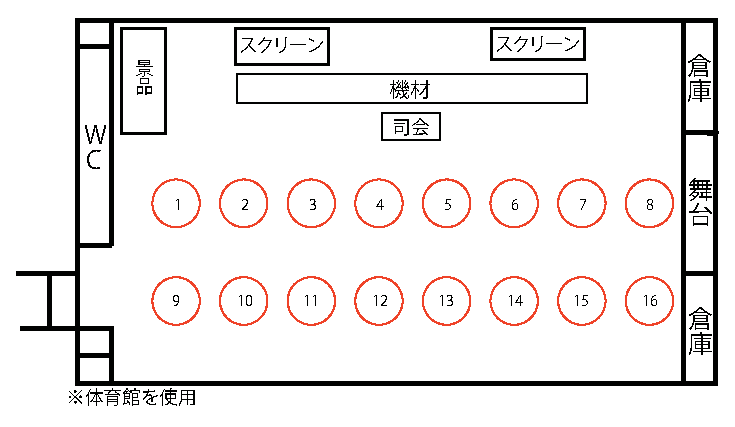
\includegraphics[width=12cm]{./21/reiout1.eps}
\label{fig:ice}

\end{center}

\subsection{物品}
